\documentclass[11pt,a4paper]{article}
\usepackage[brazil]{babel} % carrega portugues brasileiro
\usepackage[utf8]{inputenc}
\usepackage[T1]{fontenc}
\usepackage[top=2cm, bottom=2cm, left=2cm, right=2cm]{geometry} %margens menores!
\usepackage{graphicx} % incluir figuras .eps
\usepackage{tabularx}
\usepackage{color} % colorir texto
\usepackage{indentfirst}
\usepackage{textcomp}
\usepackage[colorlinks=true]{hyperref}
\usepackage{amssymb,amsmath}
\usepackage{float}
\usepackage{tablefootnote}
\usepackage{changepage}

% \usepackage[ampersand]{easylist}

\title{Interface para transmissão digital de arquivos}

\author{
       \large
        \textsc{Rafael Diniz}
        \mbox{}\\ %
        rafael@riseup.net\\
        \mbox{} %
        SDR Telecom\\
        \mbox{} %
        \normalsize
        \texttt{Departamento de desenvolvimento de interfaces}\\
}
\date{\today}


\begin{document}

\maketitle

\begin{abstract}

Este documento contém um rascunho da interface do software para transmissão
digital de arquivos via HF, padrão HamDRM.

\end{abstract}

\newpage

% \tableofcontents

\section{Fluxograma}

\begin{figure}[H]
  \centering
  \hspace*{-1cm}
  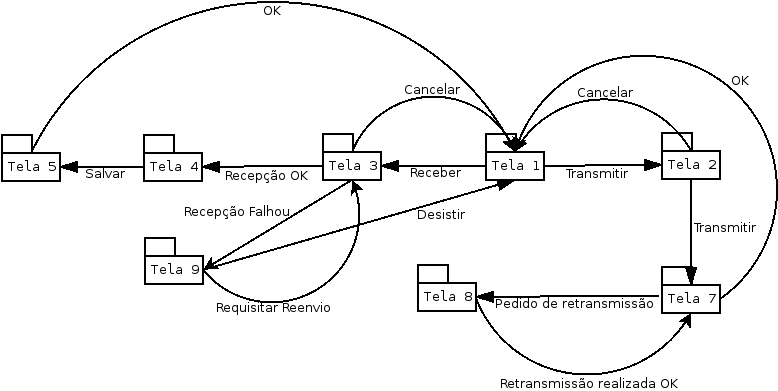
\includegraphics[scale=0.7]{Diagram.png}
  \caption{Diagrama de fluxo.}
  \label{f0}
\end{figure}

\section{Tela1}

\begin{figure}[H]
  \centering
  \hspace*{-1.5cm}
  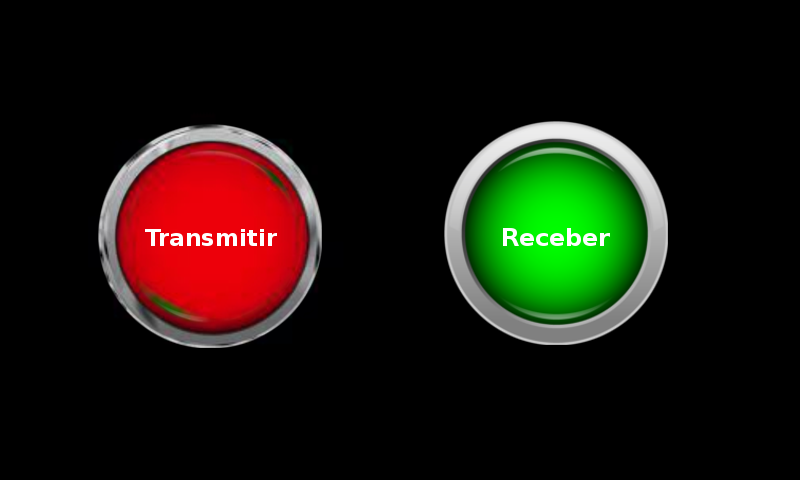
\includegraphics[scale=0.7]{Tela1.png}
  \caption{Tela 1.}
  \label{Tela1}
\end{figure}

\section{Tela2}

\begin{figure}[H]
  \centering
  \hspace*{-1.5cm}
  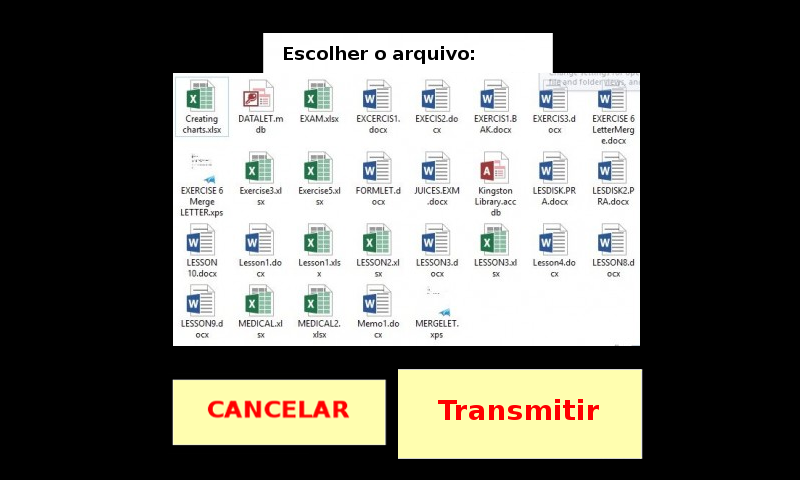
\includegraphics[scale=0.7]{Tela2.png}
  \caption{Tela 2.}
  \label{Tela2}
\end{figure}

\section{Tela3}

\begin{figure}[H]
  \centering
  \hspace*{-1.5cm}
  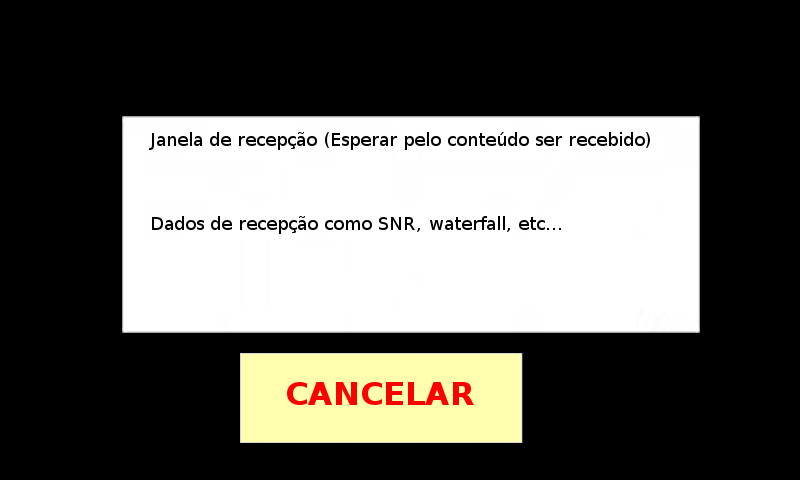
\includegraphics[scale=0.7]{Tela3.png}
  \caption{Tela 3.}
  \label{Tela3}
\end{figure}

\section{Tela4}

\begin{figure}[H]
  \centering
  \hspace*{-1.5cm}
  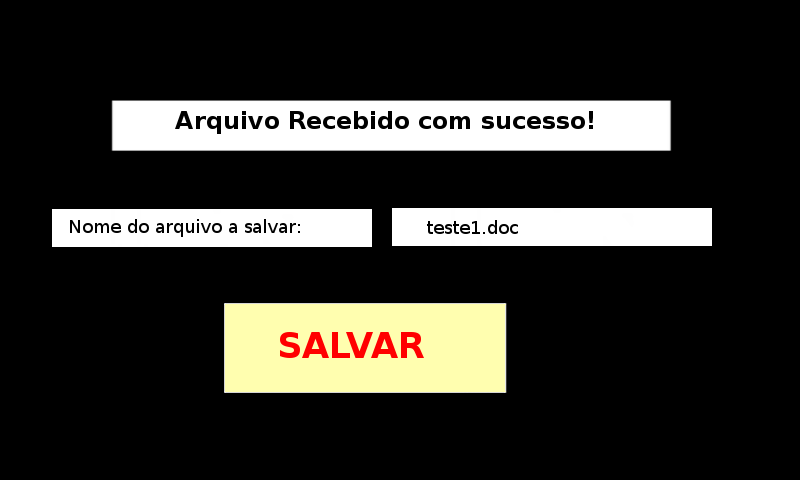
\includegraphics[scale=0.7]{Tela4.png}
  \caption{Tela 4.}
  \label{Tela4}
\end{figure}

\section{Tela5}

\begin{figure}[H]
  \centering
  \hspace*{-1.5cm}
  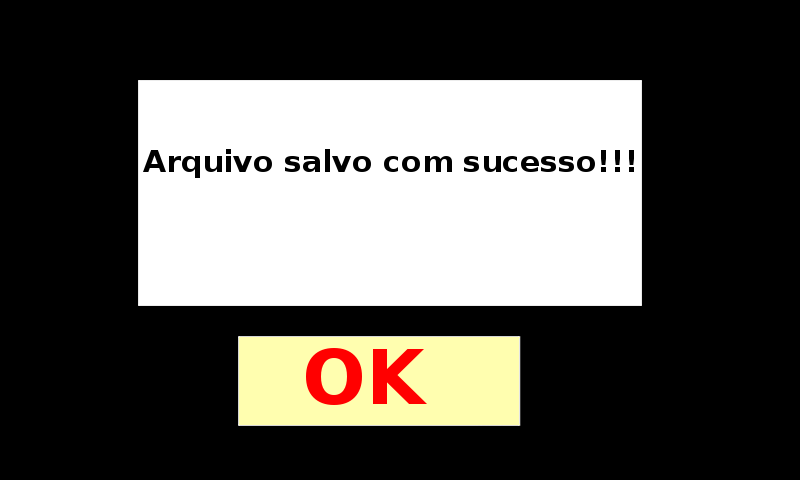
\includegraphics[scale=0.7]{Tela5.png}
  \caption{Tela 5.}
  \label{Tela5}
\end{figure}

\section{Tela6}

\begin{figure}[H]
  \centering
  \hspace*{-1.5cm}
  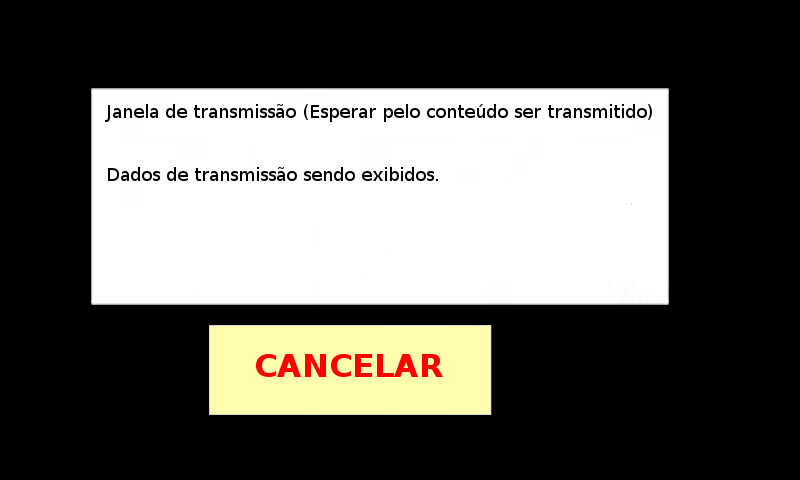
\includegraphics[scale=0.7]{Tela6.png}
  \caption{Tela 6.}
  \label{Tela6}
\end{figure}

\section{Tela7}

\begin{figure}[H]
  \centering
  \hspace*{-1.5cm}
  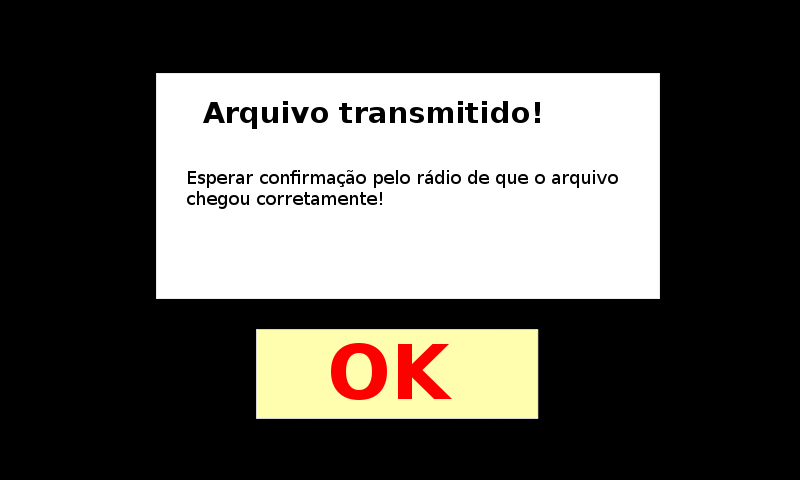
\includegraphics[scale=0.7]{Tela7.png}
  \caption{Tela 7.}
  \label{Tela7}
\end{figure}

\section{Tela8}

\begin{figure}[H]
  \centering
  \hspace*{-1.5cm}
  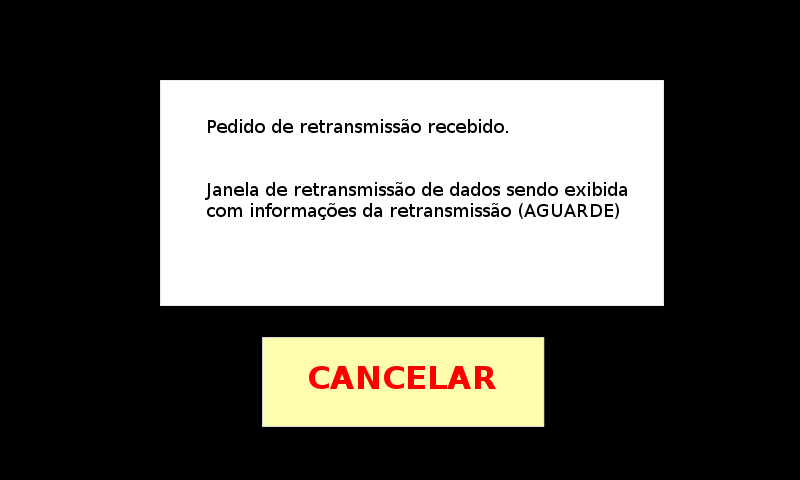
\includegraphics[scale=0.7]{Tela8.png}
  \caption{Tela 8.}
  \label{Tela8}
\end{figure}

\section{Tela9}

\begin{figure}[H]
  \centering
  \hspace*{-1.5cm}
  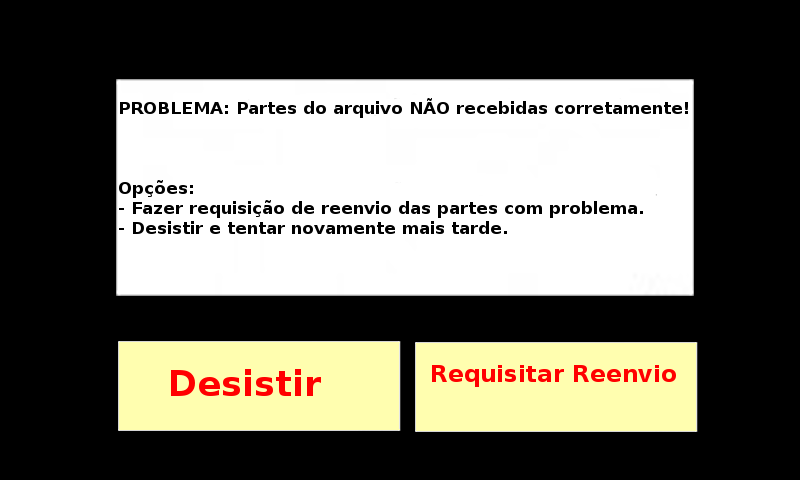
\includegraphics[scale=0.7]{Tela9.png}
  \caption{Tela 9.}
  \label{Tela9}
\end{figure}

\end{document}
